\chapter{Zespołowe przedsięwzięcie}

\begin{itemize}
\item Zespołowe przedsięwzięcie inżynierskie oznaczać będzie projekt, działanie podjęte w realizacji postawionego celu, realizowane zespołowo.

\item Projekt jest odpowiedzią na problem/potrzebę, w określonej przestrzeni życia.
\end{itemize}

\section{Członkowie zespołu z określeniem funkcji}
\begin{description}
\item[1] Piotr Jabloński - programista Java
\item[2] Mirosława Pelc - programista Java
\item[3] Mariusz Lorek - kierownik zespołu, testowanie, przygotowanie dokumentacji
\end{description}

\section{Uzasadnienie potrzeby realizacji projektu}
Potrzebny jest program który wspomoże zorganizowanie turnieju szachowego w którym może wziąść udział dowolna, nieznana wcześniej liczba zawodników. Czas trwania turnieju jest ograniczony przez organizatora. Turniej szachowy jest organizowany cyklicznie, dlatego stworzenie programu wspomagającego jego obsługę znacznie ułatwi przeprowadzanie kolejnych edycji.


\section{Cele projektu}
\begin{enumerate}
\item Stworzenie programu wspomagającego organizację turnieju szachowego.
Napisany program ma pozwolić na sprawne przeprowadzenie turnieju szachowego i wyłonienie zwycięzcy turnieju i/lub zawodników którzy zajeli kolejne miejsca w turnieju.
\item Przygotowanie instrukcji obsługi programu/aplikacji dla użytkownika końcowego
\end{enumerate}
 


\section{Zakres projektu}
\begin{enumerate}
	\item Stworzenie programu do wspomagania organiacji turnieju szachowego według wytycznych zleceniodawcy
	\item Stworzenie dokumentacji opisującej postępy prac nad tworzonym projektem z podziałem na czynności które ma wykonywać każdy z członków zespołu
\end{enumerate}
Gotowy program ma pozwalać m.in na:
\begin{itemize}
	\item  przeprowadzenie turnieju szachowego w systemie szwajcarskim 
	\item zarzadzanie turniejami w bazie danych 
	\item zgromadzenie podstawowych danych o zawodnikach, jakim są: (Imię, Nazwisko, Wiek, Kategoria szachowa) 
	\item dodawanie, usuwanie i edycja zawodników, 
	\item podział zawodników na grupy w ze względu na przedział wiekowy, kategorie szachową lub manualnie. 
	\item ustalenie liczby grup oraz szachownic przed rozpoczęciem nowego turnieju. 
	\item ustalanie uczestników każdego meczu - kolor pionków (biały, czarny) przydzielany do zawodników przed każdym spotkaniem 
	\item punktowanie rozegranych spotkań
\end{itemize}


\section{Grupy docelowe}
Program przeznaczony dla organizatorów turniejów szachowych.  


\section{Struktura podziału prac (zadań) - WBS}

\begin{example}
Program wspomagający przeprowadzenie turneju szachowego
\begin{enumerate}
\item Zebranie informacji na temat sposobu przprowadzania turnieju szachowego od zleceniodawcy
\begin{enumerate}
	\item Wybranie systemu według którego będzie przeprowadzany turniej, wybór najoptymalniejszego rozwiązania
	\item Przygotowanie regulaminu turnieju.
\end{enumerate}
\item Projekt programu
\begin{enumerate}
\item Określenie jakie elementy muszą się znaleść w programie
\item Szablon programu
\item Wybór narzędzi/aplikacji służących do napisania programu
\item Rozdzielenie zadań dla programistów
\end{enumerate}
\item Tworzenie programu/aplikacji
\begin{itemize}
\item Opracowanie narzędzi bazodanowych przechowujących informacje dotyczące turniejów
\item Przygotowanie elementów środowiska graficznego
\item Integracja narzędzi bazodanowych z elementami środowiska graficznego

\item Wstępna wersja programu
\item Testowanie
\begin{enumerate}
	\item Weryfikacja - "Czy budujemy prawidłowo produkt", dynamiczna i statyczna
	\item Walidacja - "Czy budujemy prawidłowy produkt"
	\item Testy
	\begin{itemize}
		\item Testy jednostkowe
		\item Testy integracyjne
		\item Testy systemowe
		\item Testy użyteczności
		\item Testy akceptacyjne (przeprowadzane przez zleceniodawce projektu
	)
	Testy mają za zadanie sprawdzenie każdego komponentu nieza
	\end{itemize}
\end{enumerate}
\item Eliminacja znalezionych błędów
\item Dodawanie kolejnych funkcji do programu

\end{itemize}
\item Końcowa wersja programu

\end{enumerate}
\end{example}

\section{Regulamin turnieju}
\begin{enumerate}
	\item Obowiązują przepisy gry miedzynarodowej federacji szchowej (FIDE).
	\item Podczas turnieju obowiązuje system kołowy, każdy z każdym \url{http://www.pzszach.org.pl/index.php?idm=4&idm2=125&idm3=217}
	\begin{enumerate}
		\item Podstawowe zasady rozgrywania turnieju
		\\Podstawowe zasady prowadzenia turniejów są następujące:
\begin{enumerate}
\item Zawodnicy dzieleni są na grupy według wybranych kryteriów
\item Zawodnicy mogą grać przeciwko sobie tylko jeden raz w trakcie turnieju. 
\item Jeśli jest to możliwe, to zawodnik powinien grać tę samą liczbę partii białymi i czarnymi bierkami. 
\item Jeśli jest to możliwe, to zawodnik powinien zachować prze-mienność kolorów bierek w kolejnych rozgrywkach
\item Końcowa klasyfikacja turnieju wynika z sumy uzyskanych punktów, licząc 1 punkt za zwycięstwo, 0,5 punktu za remis i 0 punktów za przegraną. Zawodnik, którego przeciwnik nie stawił się do gry, otrzymuje 1 punkt.
\end{enumerate}
\item \textbf{Pauzowanie}
\begin{enumerate}
	\item W przypadku nieparzystej liczby uczestników w jakiejkolwiek rundzie, powinien pauzować zawodnik z najniższym numerem startowym, w najniższej grupie punktowej
	\item Zawodnik może pauzować tylko jeden raz w trakcie tur-nieju. Jeżeli otrzymał walkower w poprzednich rundach, nie może być wyznaczony do pauzowania w następnych.
	\item Pauzujący zawodnik otrzymuje jeden punkt w danej run-dzie. Nie miał on jednak w tej rundzie przeciwnika, więc nie otrzymuje w danej rundzie przydziału koloru bierek.
\end{enumerate}
	\end{enumerate}
	\item Każdy z zawodników powinien się kierować zasadami fair play.
	\item W razie rezygnacji lub wykluczenia zawodnika z turnieju, rozgrywki, które zagrał nie zostają anulowane, a osoby, które się z nim spotykają w dalszych rozgrywkach wygrywają walkowerem 
	\item Zawodnicy, którzy nie grają lub czekają na swoją kolej w obrębie sali lub w niedalekiej odległości od niej w wypadku wezwania do rozgrywki powinni w trybie natychmiastowym zgłosić się do udziału w spotkaniu. W wypadku niestawienia się do rozegrania meczu zawodnik zostaję zdyskwalifikowany.
	\item W przypadku, gdy:
\begin{itemize}
	\item Zawodnik utrudnia przeprowadzanie rozgrywek może zostać zdyskwalifikowany z turnieju lub wyproszony z sali przez Prowadzącego.
	\item Widz utrudnia przeprowadzanie rozgrywek może zostać wyproszony z sali przez Prowadzącego.
\end{itemize}
\item Udział w turnieju szachowym jest równoznaczny z zaakceptowaniem regulaminu
\end{enumerate}
\section{Diagram sieciowy}
Diagram sieciowy ukazuje zależności czasowe, węzły (aktywności), krawędzie (zależności czasowe).


\section{Harmonogram}
\subsection{Harmonogram prac poszczególnych członków zespołu}
\textbf{Mirosława Pelc oraz Piotr Jabłoński wspólna praca programistyczna\\
Mirosława Pelc - Odpowiedzialna w głównej mierze za interfejs graficzny\\
Piotr Jabłoński - Programowanie, algorytmy\\}
\begin{enumerate}
\item Przygotowanie klas odpowiadających za uczestnika, turniej, rozgrywkę - 20.10.2015
\item wyszukikawanie możliwych do wykorzystania elementów dostępnych w bibliotekach graficznych dla języka JAVA 20.10.2015 - zadanie ciągłe wykonywane przez cały czas trwania projektu\\

\item integracja z bazą danych SQLite do przechowywania uczestników - 27.10.2015
\item integracja z bazą danych SQLite do przechowywania turniejów - 27.10.2015
\item integracja z bazą danych SQLite do przechowywania wyników pojedynczych rozgrywek - 27.10.2015\\

\item tabela - lista uczestników - 3.11.2015
\item dodawanie nowego uczestnika - 3.11.2015\\

\item usuwanie uczestnika - 10.11.2015
\item edycja uczestnika - 10.11.2015\\

\item dodawanie losowego uczestnika - 17.11.2015
\item symulacja ilości rozgrywek dla danej liczby uczestników, typu turnieju (systemem szwajcarskim / eliminacje grup) - 17.11.2015\\


\textbf{DO ZROBIENIA\\}

\item podział graczy na grupy wg listy sortowanej po ustalanych przez prowadzącego turniej (dynamicznie w programie) warunkach 
takich, jak: kategoria zawodnika, wiek, nazwisko, imię lub przydział manualny - 24.11.2015
\item tworzenie początkowej listy graczy (sortowanie) do turnieju rozgrywanego systemem szwajcarskim 
(sortowanie po kategorii, wieku, nazwisko, imię) - 24.11.2015\\

\item dobieranie zawodników w pary dla systemu kołowego z eliminacjami w grupach - eliminacje
wybór zawodników przechodzących do finałów w rozgrywkach z eliminacjami
dobieranie zawodników w pary dla systemu kołowego z eliminacjami w grupach - finały
\item dobór zawodników w systemie kołowym (4 tyg!)
\item lista wyników dla turnieju rozgrywanego systemem kołowym z eliminacjami 
\item lista wyników dla turnieju rozgrywanego systemem szwajcarskim 
\item zastosowanie programu do prowadzednia kilku turniejów jednocześnie
\item usprawnienia ergonomii interfejsu
\item usprawnienia estetyczne interfejsu
\end{enumerate}

\textbf{Mariusz Lorek:}
\begin{enumerate}
	\item Przygotowanie dokumentacji dla projektu - cały czas trwania projektu
	\item Rozmowa ze zleceniodawcą na temat projektu 20.10.2015
	\item Wybór systemu w którym przeprowadzany będzie turniej 27.10.2015
	\item Okreslenie regulaminu turnieju (czas trwania,  system rozgrywego, określenie zasad uczestnictwa w turnieju, powody do dyskwalifikacji) 3.11.2015
	\item Przygotowywanie kolejnych części dokumentacji na podstawie informacji dostarczonych przez pozostałych członków zespołu

\end{enumerate}


\section{Dokumentacja}
Przygotowanie środowiska do równoległego opracowania dokumentacji projektu i realizacji przydzielonych zadań poszczególnym członkom zespołu projektowego.

\subsection[Edycja plików dokumentacyjnych]{Edycja plików dokumentacyjnych - każdy członek zespoły niezależnie}
Każdy z członków zespołu edytuje swój plik \LaTeX{} (czlonkowie/nrCzlonka/main.tex) i~umieszcza w nim całość analiz i wyników, które pozwoliły mu zrealizować przydzielone zadanie. Wszystkie pliki graficzne, każdy niezależnie umieszcza w swoim katalogu (czlonkowie/nrCzlonka).

Pierwszą linia w pliku (czlonkowie/nrCzlonka/main.tex), zawiera imię i nazwisko opracowującego członka zespołu:
\begin{lstlisting}
\osoba{Jan Iksiński}
\end{lstlisting}

Każde działanie/zadanie należy DOKŁADNIE opisać podając w poleceniu \s!\zadanieprojektowe! cztery obowiązkowe dane:
\begin{itemize}
\item Rodzaj zadania [Przygotowanie przestrzeni do zespołowej pracy]
\item Data rozpoczęcia [2014-11-01]
\item Data zakończenia [2014-11-02]
\item Aktualny status [zaplanowane do realizacji, w trakcie realizacji, zakończone]
\item dokładny opis realizowanego zadania [powinien zawierać opis, rysunki, tabele, kody napisanych programów]
\end{itemize}

Poniżej znajduje się przykładowy listing dla skróconych dwóch zadań:
\begin{lstlisting}
\zadanieprojektowe{Przygotowanie dokumentacji}{2014-11-01}{2014-11-02}{w trakcie do realizacji}

Poniżej opisujemy całe zadanie zgodnie z konwencją poznaną na NI.
Poniżej opisujemy całe zadanie zgodnie z konwencją poznaną na NI.

Poniżej opisujemy całe zadanie zgodnie z konwencją poznaną na NI. 

%następne zadanie
\zadanieprojektowe{Przygotowanie dokumentacji}{2014-11-03}{2014-11-03}{zakończone}
\begin{figure}[H]
\includegraphics[width=\textwidth]{czlonkowie/1/studzienkizDziura.jpg}
\end{figure}
\end{lstlisting}


\subsubsection{Obsługa GitHuba}
Repozytorium wykorzystywane w projekcie to "GitHub" aby zacząć korzystać z tego repozytorium należy najpierw założyć konto w serwisie \href{https://github.com}{https://github.com}
Wybieramy opcję "Sing up" i wypełnamy formularz rejestracyjny
\begin{figure}
	\centering
	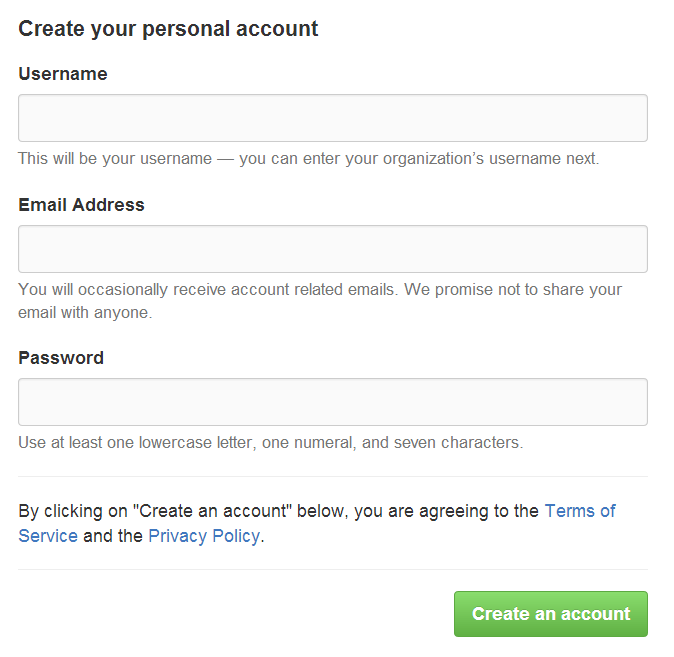
\includegraphics {fig/rejestracja}
	\caption{Formularz rejestracyjny repozytorium GitHub}
	\label{fig:rejestracja}
\end{figure}
Nastepnie z menu na górze po prawej stronie wybieramy opcję "New repository"
\begin{figure}
	\centering
	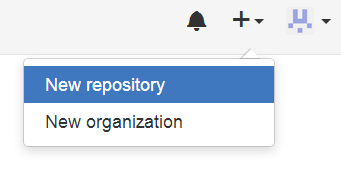
\includegraphics{fig/new_project}
	\caption{Tworzenie nowego repozytorium}
	\label{fig:new_project}
\end{figure}
Uzupełniamy dane dotyczące projektu. Musimy mu nadać nazwę, możemy opcjonalnie dodać opis tworzonego repozytorium, oraz zdecydować czy projekt będzie publiczny czy prywatny

\begin{figure}
	\centering
	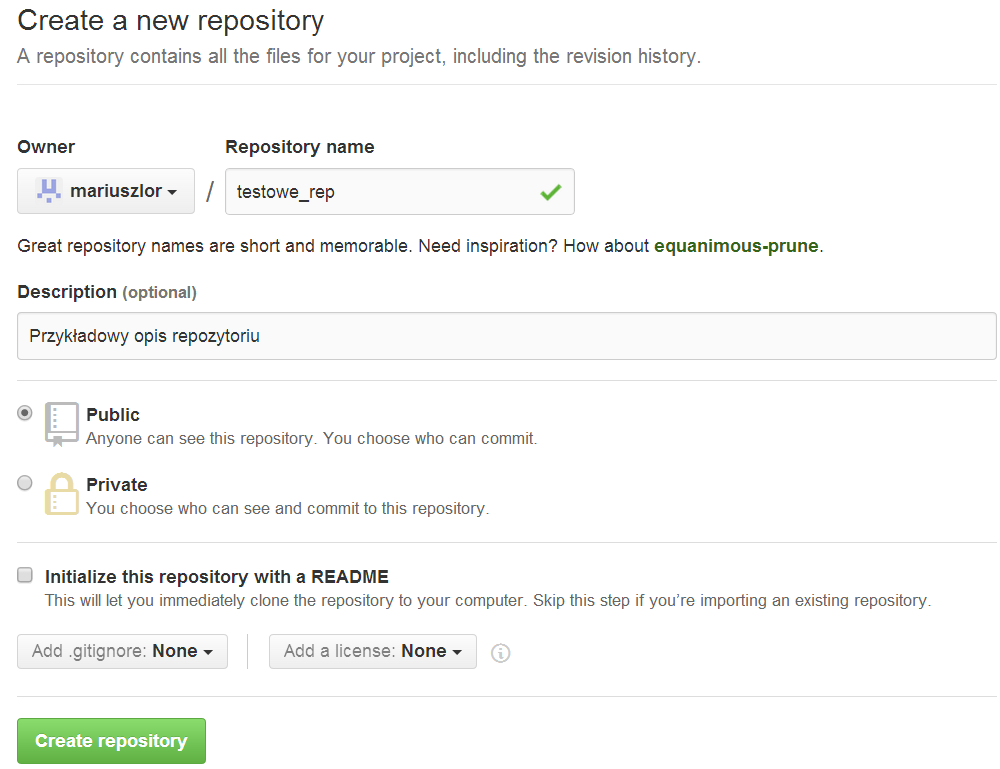
\includegraphics{fig/new_project_2}
	\caption{Uzupełniamy dane na temat projektu}
	\label{fig:new_project2}
\end{figure}
Teraz możemy dodać kolejnych uczestników projektu wybierając z menu opcję "New collaborator"
Uczestników możemy wyszukiwać  według róznych kryteriów
\begin{figure}
	\centering
	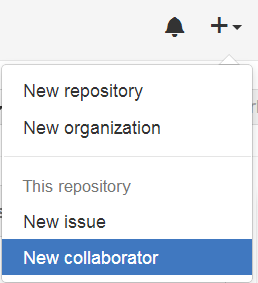
\includegraphics{fig/collaborator}
	\caption{Dodawanie nowego uczestnika projektu}
	\label{fig:collaborator}
\end{figure}
\begin{figure}
	\centering
	
\includegraphics{fig/add_collaborator}
	\caption{Mamy możliwość wyszukiwania nowych członków według różnych kryteriów}
	\label{fig:add_collaborator}
\end{figure}
